\documentclass{article}
\usepackage{fullpage}
\usepackage{graphicx}
\usepackage{url}
\begin{document}

\title{XBP User Guide}

\maketitle

\begin{figure}[ht]
  \begin{center}
    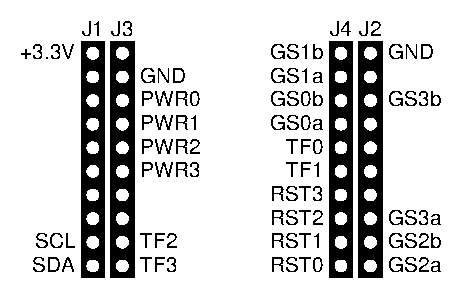
\includegraphics[scale=1]{figures/xbp-xbh}
    \caption{Boosterpack Connector XBH as Viewed from Top}
  \end{center}
\end{figure}

\begin{figure}[ht]
  \begin{center}
    \includegraphics[scale=1]{figures/xbp-xbd}
    \caption{Boosterpack Connector XBD as Viewed from Top}
  \end{center}
\end{figure}
\begin{table}[ht]
  \begin{center}
    \caption{Pin Configuration of Boosterpack Connector for XBH}
    \begin{tabular}{rlll}
      Connector & Pin  & Net         & Comment  \\ \hline
       J1 & 1  & +3V3      & Supply Voltage from XBH for I$^2$C pullup resistors on XBP0 \\
       J1 & 9  & SCL       & I$^2$C Serial Clock  \\
       J1 & 10 & SDA       & I$^2$C Serial Data \\ \hline

       J3 & 23 & PWR0      & Analog signal of current consumption of XBD0 from XBP0\\
       J4 & 37/38 & GS0a/GS0b & Gain select for current monitor of XBD0 on XBP0\\
       J4 & 36 & TF0       & Timer Flag from XBD0 \\
       J4 & 31 & RST0      & Reset of XBD0 \\ \hline

       J3 & 24 & PWR1      & Analog signal of current consumption of XBD1 from XBP1 \\
       J4 & 39/40 & GS1a/GS1b & Gain select for current monitor of XBD1 on XBP1\\
       J4 & 35 & TF1       & Timer Flag from XBD1 \\
       J4 & 32 & RST1      & Reset of XBD1 \\ \hline

       J3 & 25 & PWR2      & Analog signal of current consumption of XBD2 from XBP2 \\
       J2 & 11/12 & GS2a/GS2b & Gain select for current monitor of XBD2 on XBP2\\
       J3 & 29 & TF2       & Timer Flag from XBD2 \\
       J4 & 33 & RST2      & Reset of XBD2 \\ \hline

       J3 & 26 & PWR3      & Analog signal of current consumption of XBD3 from XBP3 \\
       J2 & 13/18 & GS3a/GS3b & Gain select for current monitor of XBD3 on XBP3\\
       J3 & 30 & TF3       & Timer Flag from XBD3 \\
       J4 & 34 & RST3      & Reset of XBD3 \\ \hline

       J2 & 20 & GND       & \\
       J3 & 22 & GND       & \\ \hline
    \end{tabular}
  \end{center}
\end{table}
\begin{table}[ht]
  \begin{center}
    \caption{Pin Configuration of Boosterpack Connector for XBD}
    \begin{tabular}{rlll}
      Connector & Pin  & Net         & Comment  \\ \hline
       J1 & 1  & +3V3      & Supply Voltage, current is measured by XBP \\
       J1 & 9  & SCL       & I$^2$C Serial Clock  \\
       J1 & 10 & SDA       & I$^2$C Serial Data \\
       J2 & 16 & RST       & Reset of XBD \\ 
       J2 & 19 & TF        & Timer Flag to start/stop execution timer on XBH \\
       J2 & 20 & GND       & \\
       J3 & 22 & GND       & \\ \hline
    \end{tabular}
  \end{center}
\end{table}


\end{document}
